%
% MIT License
%
% Copyright (c) 2024 Fabricio Batista Narcizo.
%
% Permission is hereby granted, free of charge, to any person obtaining a copy
% of this software and associated documentation files (the "Software"), to deal
% in the Software without restriction, including without limitation the rights
% to use, copy, modify, merge, publish, distribute, sublicense, and/or sell
% copies of the Software, and to permit persons to whom the Software is
% furnished to do so, subject to the following conditions:
%
% The above copyright notice and this permission notice shall be included in
% all copies or substantial portions of the Software.
%
% THE SOFTWARE IS PROVIDED "AS IS", WITHOUT WARRANTY OF ANY KIND, EXPRESS OR
% IMPLIED, INCLUDING BUT NOT LIMITED TO THE WARRANTIES OF MERCHANTABILITY,
% FITNESS FOR A PARTICULAR PURPOSE AND NONINFRINGEMENT. IN NO EVENT SHALL THE
% AUTHORS OR COPYRIGHT HOLDERS BE LIABLE FOR ANY CLAIM, DAMAGES OR OTHER
% LIABILITY, WHETHER IN AN ACTION OF CONTRACT, TORT OR OTHERWISE, ARISING FROM,
% OUT OF OR IN CONNECTION WITH THE SOFTWARE OR THE USE OR OTHER DEALINGS IN THE
% SOFTWARE.
%

% Methodology Chapter.
\chapter{Methodology}\label{chap:methodology}
\lettrine[lines=3]{T}{he} methodology chapter describes the approaches, tools, and processes you used to conduct your research. It should provide sufficient detail for the reader to understand how you gathered and analyzed data, making it possible for others to replicate your study if needed. This chapter demonstrates the rigor and validity of your research.

Start this chapter with a brief explanation of its purpose. Provide a roadmap for the reader. For example: ``\textit{This chapter outlines the research design, data collection methods, implementation details, evaluation metrics, and ethical considerations of this study. It provides a comprehensive explanation of the processes used to address the research questions presented in Section~\ref{sec:research-questions}}.''

\section{Research Design and Approach}\label{sec:research-design}
Describe the overall design of your study. Explain whether it is experimental, observational, qualitative, or quantitative, and justify why this approach is appropriate for addressing your research questions.

If necessary, you can include figures or diagrams to illustrate the research design. You might include a flowchart showing the sequence of steps in your study or a diagram of the experimental setup. You must insert figures after you cited them in the text, and their captions should be below the them. There are two alternatives to include figures in your document: 1) a single figure or 2) a figure with subfigures. The former is used when you want to include a single image, while the latter is used when you want to include multiple images in a single figure. For example, Figure~\ref{fig:flow-diagram} shows the diagram of a binocular eye feature detector that I developed during my Ph.D. research project~\cite{Narcizo2017}.
\begin{figure}[htbp]
    \centering
    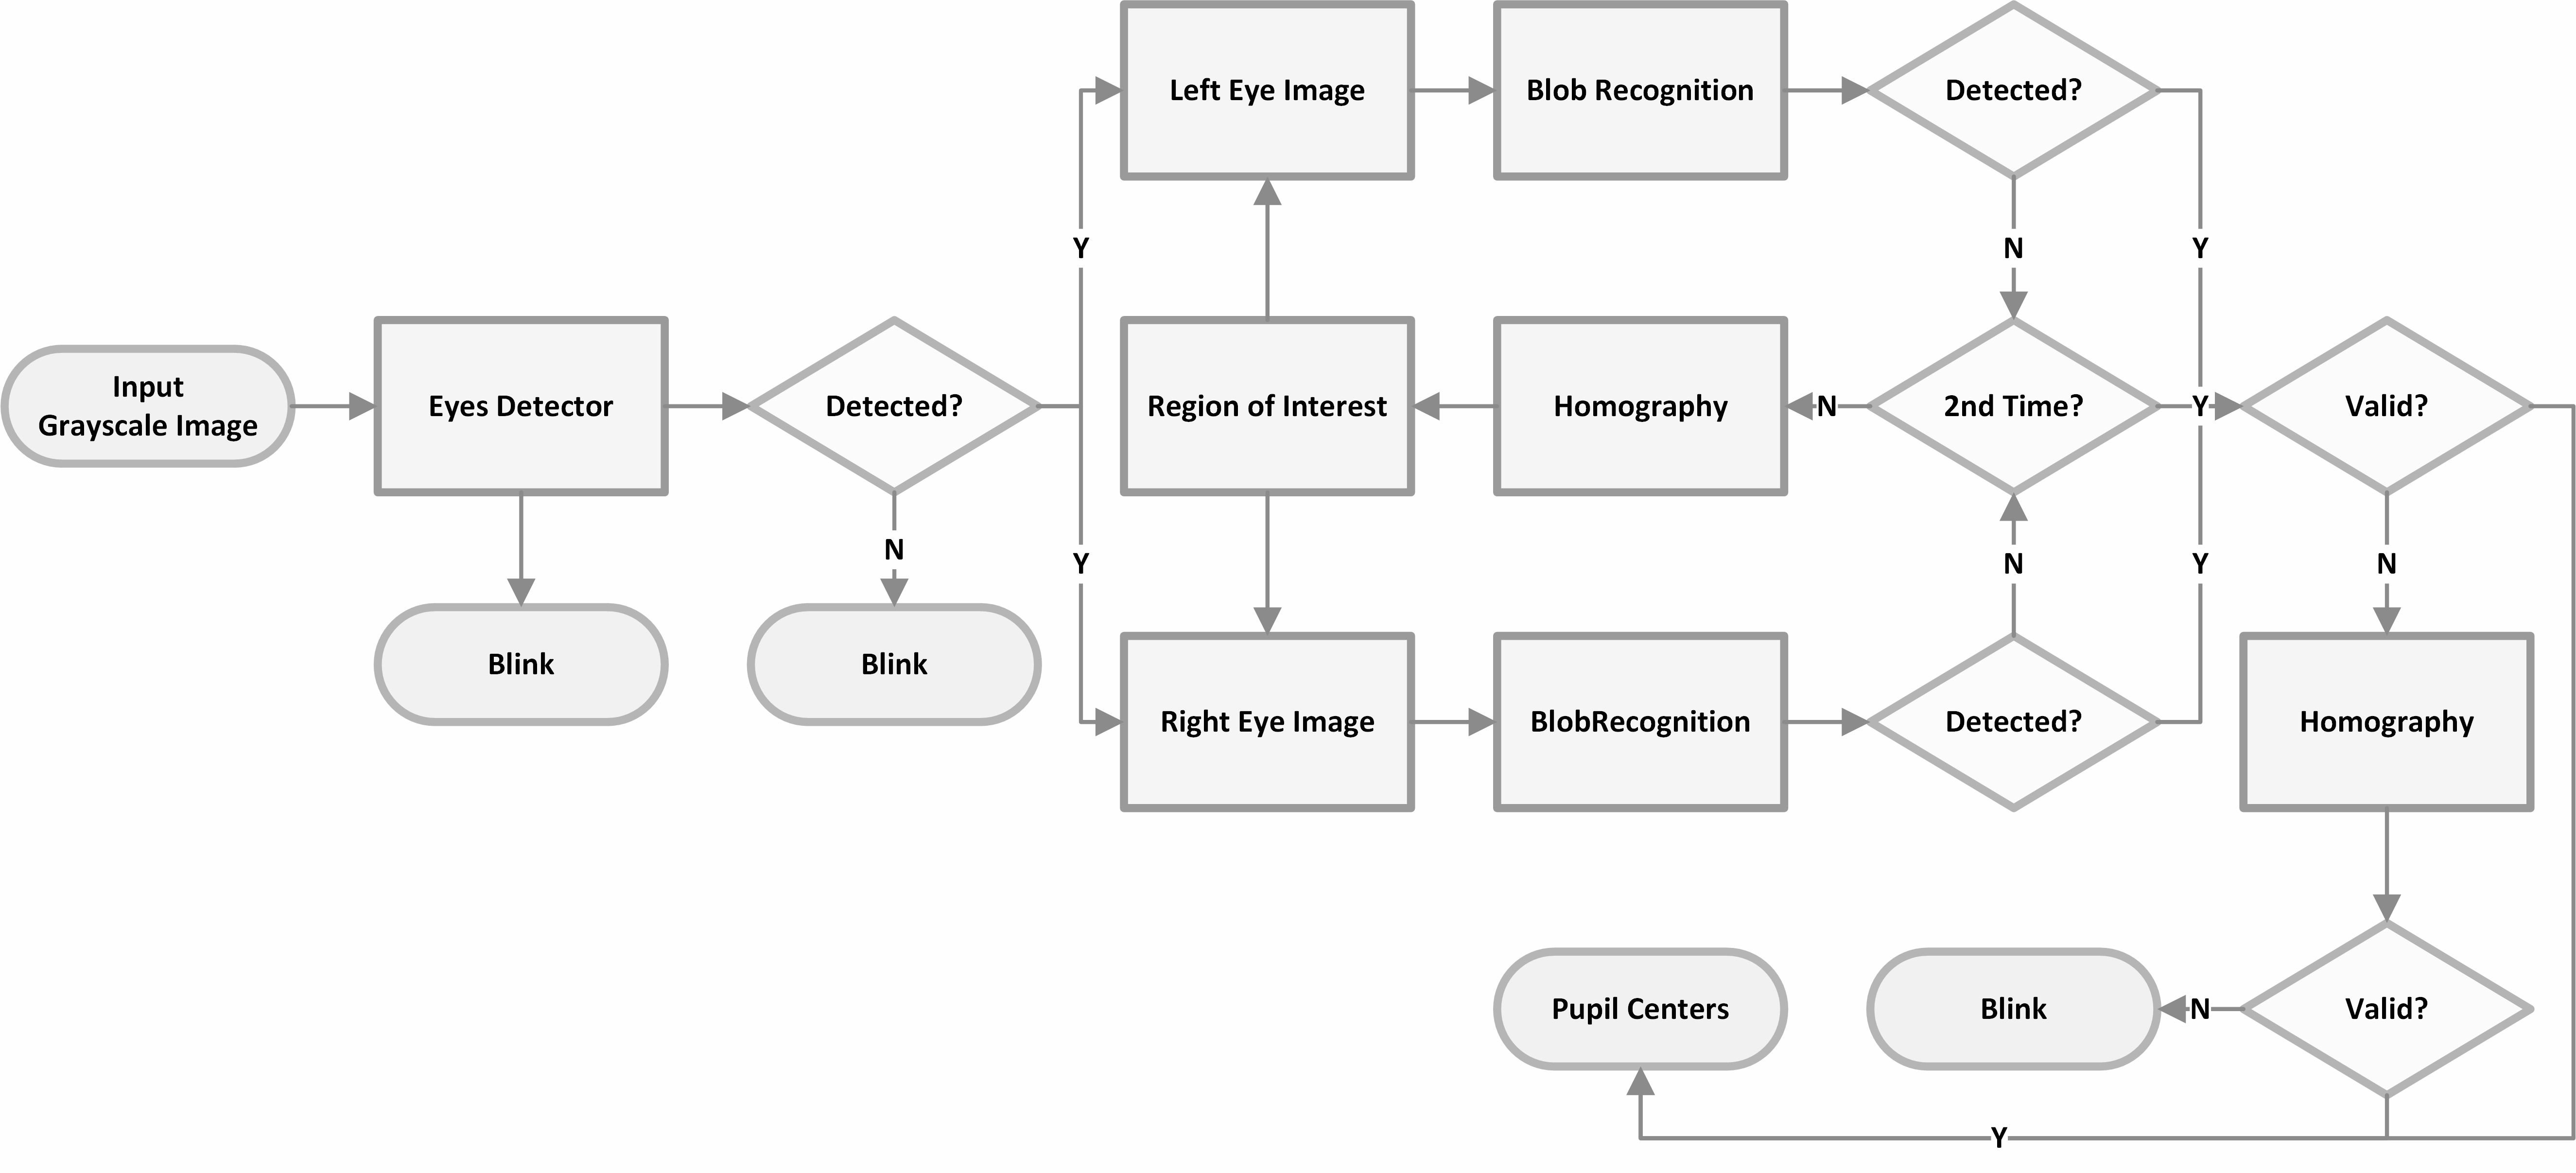
\includegraphics[width=0.8\linewidth]{flow-diagram.png}
    \caption{The proposed eye feature detector using information from both eyes}
    \label{fig:flow-diagram}
\end{figure}

On the other hand, Figure~\ref{fig:sub-figures} shows an example of a figure with subfigures. This figure includes two images side by side, each with its own caption. You can use subfigures to present related images or data together in a single figure. Figure~\ref{fig:sub-figure-a} shows an off-the-shelf head-mounted eye tracker I built during my Ph.D. research project, while Figure~\ref{fig:sub-figure-b} shows a participant of kayak experiments I performed to collect eye-tracking data of elite kayak/canoe athletes.
\begin{figure}[!ht]
    \centering
    \begin{subfigure}[b]{0.49\textwidth}
        \caption{This is the first subfigure}
        \label{fig:sub-figure-a}
        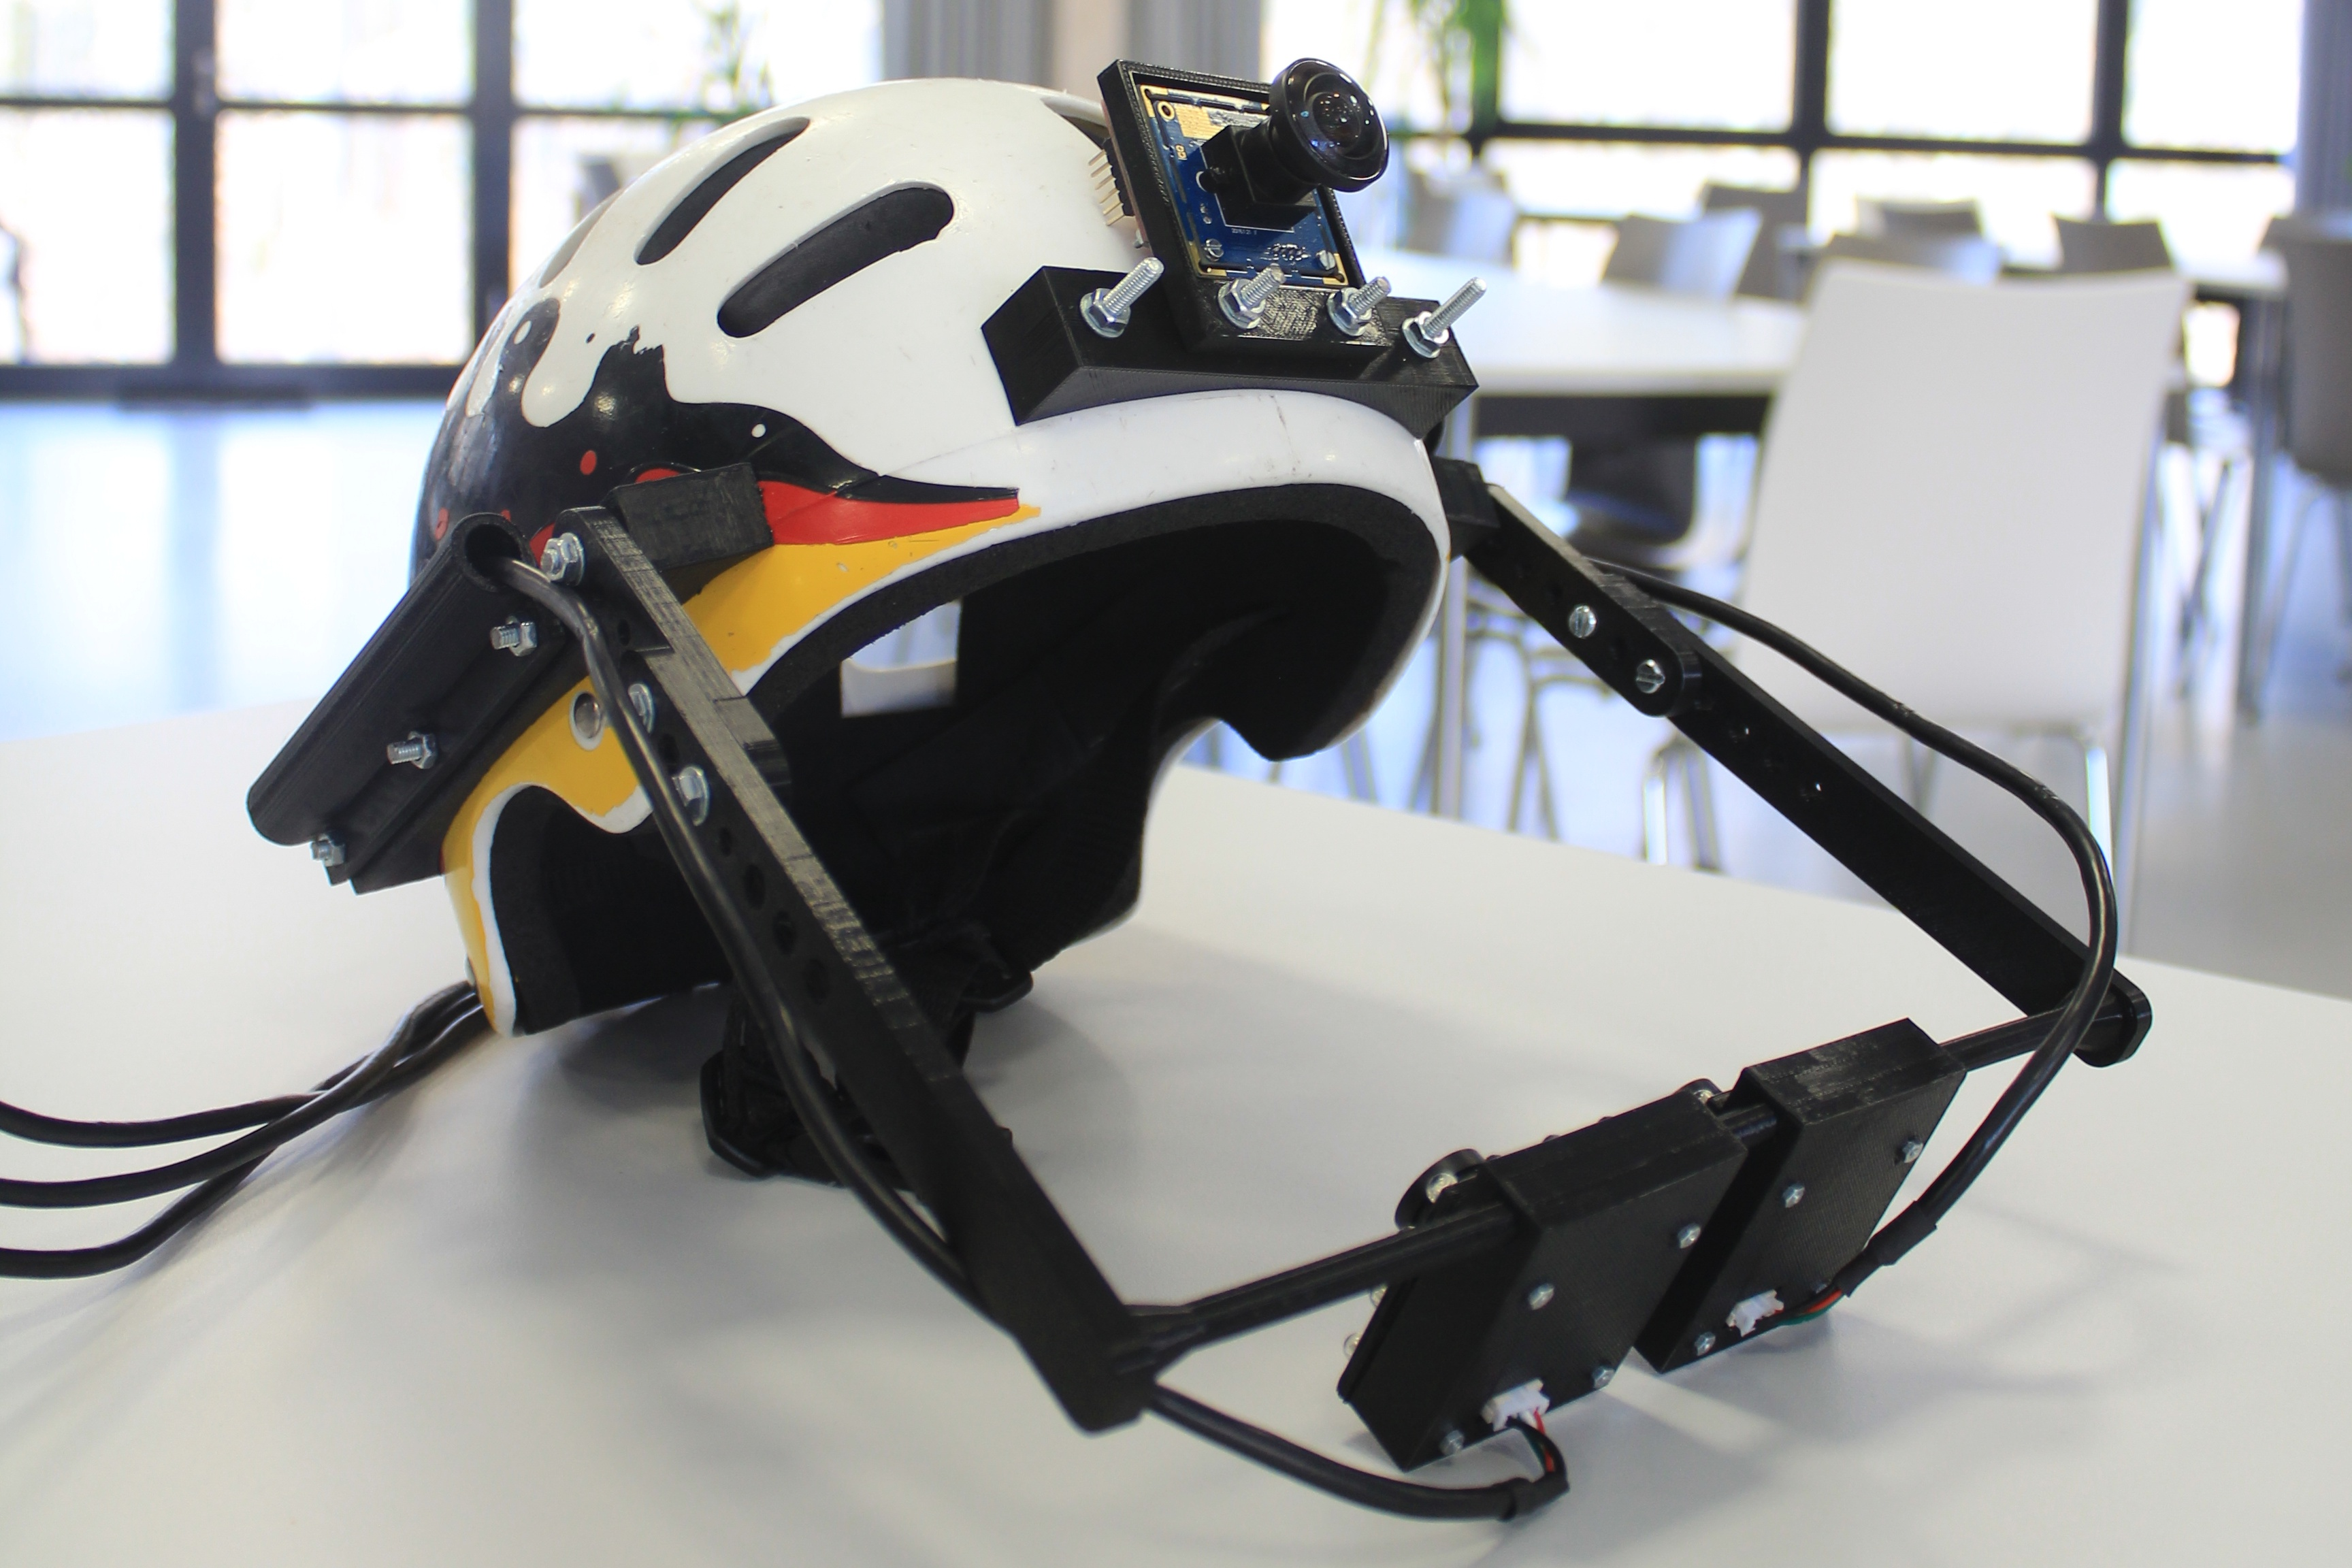
\includegraphics[width=1\linewidth]{kayak_hmet01.jpg}
    \end{subfigure}
    \begin{subfigure}[b]{0.49\textwidth}
        \caption{This is the second subfigure}
        \label{fig:sub-figure-b}
        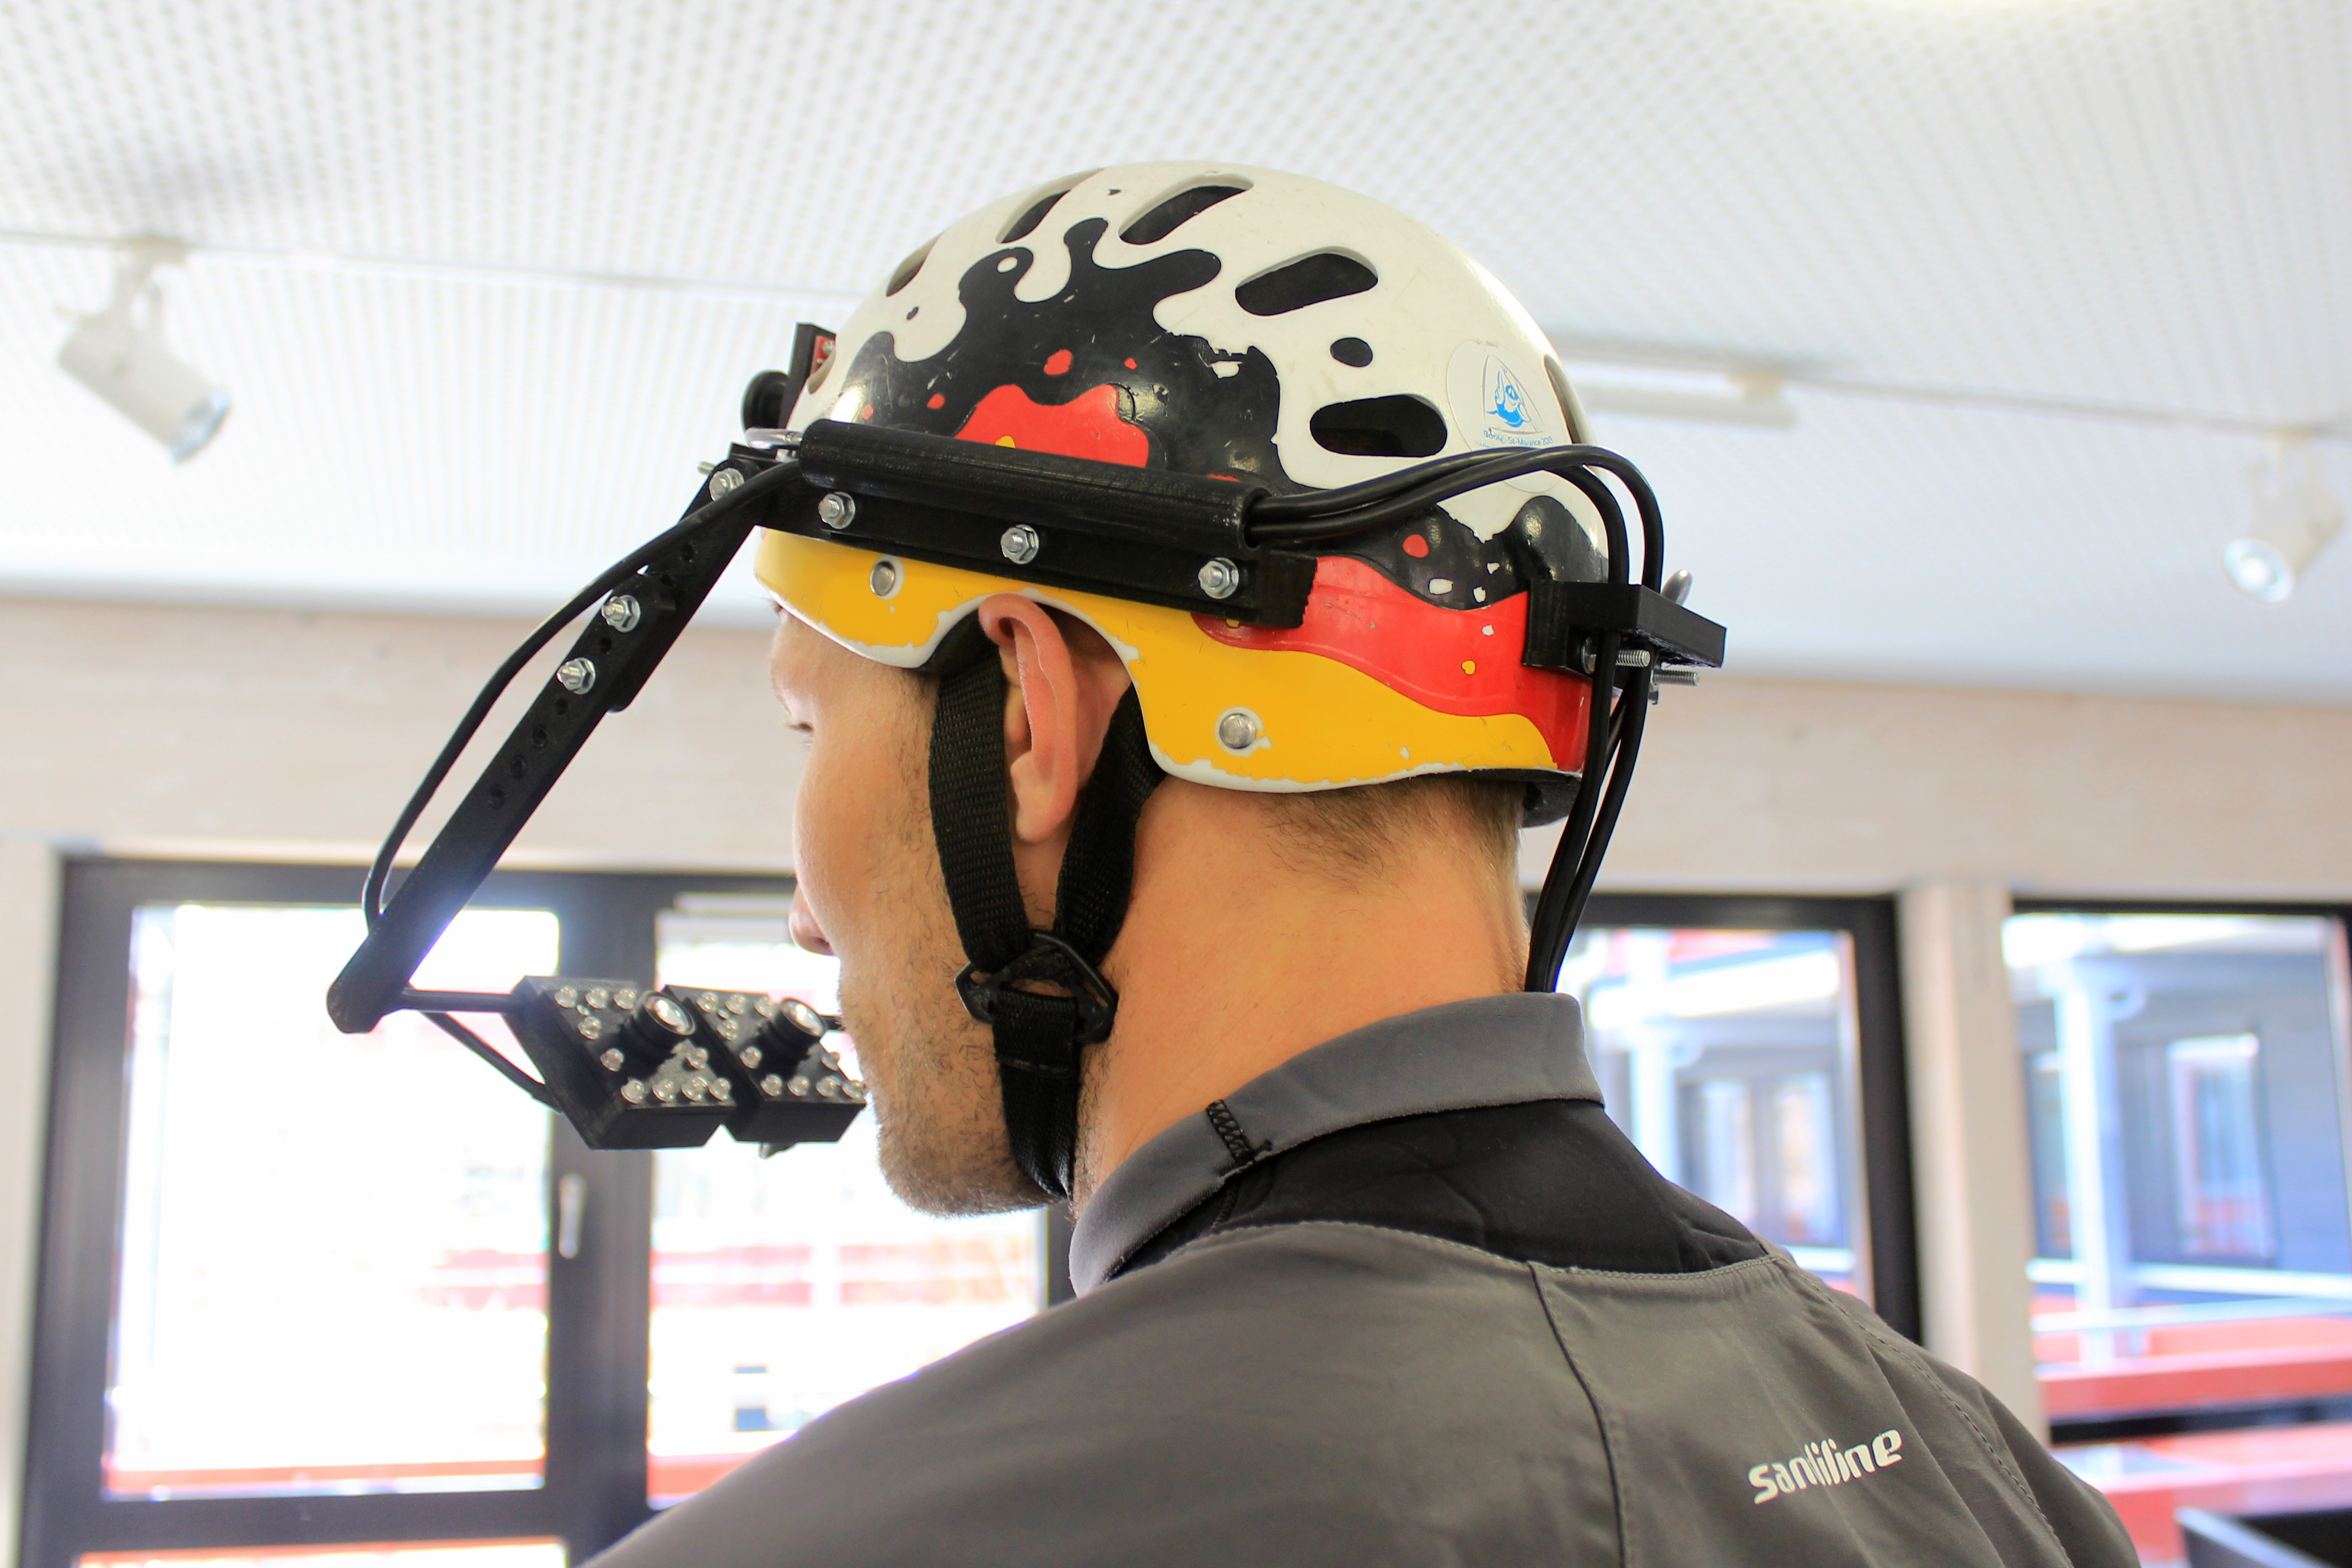
\includegraphics[width=1\linewidth]{kayak_hmet02.jpg}
    \end{subfigure}
    \caption{A head-mounted eye tracker prototype built with off-the-self hardware in a kayak helmet}
    \label{fig:sub-figures}
\end{figure}

\section{Data Collection}\label{sec:data-collection}
Provide a detailed description of how data was collected, including the datasets, tools, or systems used. Explain the sampling strategy, data sources, and data collection methods. If you conducted experiments, describe the experimental setup and procedures.

For example, you might write: ``\textit{Data was collected from 100 participants using an online survey tool. Participants were recruited through social media advertisements and were asked to complete a series of tasks related to the study. The survey included Likert scale questions, open-ended responses, and demographic information.}''

\subsection{Description of Datasets, Tools, or Systems Used}\label{subsec:datasets-tools}
Include details about the datasets, their sources, and preprocessing steps if any. Mention tools or platforms you used, such as APIs, software, or hardware. For example: ``\textit{We collected data from the Twitter API using Python scripts. The dataset consisted of 10,000 tweets related to the topic of interest. We preprocessed the data by removing duplicates and filtering out irrelevant tweets.}''

If necessary, you can include tables to present data collection details. Tables are useful for organizing large amounts of data in a structured format. For example, Table~\ref{tab:participants} shows a summary of the demographic information of the participants in the study.
\begin{center}
    \begin{threeparttable}[htbp]
        \caption{Summary of the demographic information of the participants in the study}
        \label{tab:participants}
        \begin{tabular}{cccc}
            \toprule
                \textbf{Participant ID\tnote{*}} & \textbf{Age\tnote{\textdagger}} & \textbf{Gender\tnote{\textdaggerdbl}} & \textbf{Occupation} \\
            \midrule
                1 & 25 & Female & Student \\
                2 & 30 & Male & Engineer \\
                3 & 22 & Female & Designer \\
                4 & 28 & Male & Teacher \\
                5 & 35 & Female & Scientist \\
                6 & 40 & Male & Manager \\
                7 & 27 & Female & Developer \\
                8 & 32 & Male & Analyst \\
                9 & 29 & Female & Researcher \\
                10 & 31 & Male & Consultant\tnote{\S} \\
            \bottomrule
        \end{tabular}
        \begin{tablenotes}
            \footnotesize
            \item[*] Participant ID is used to identify each participant.
            \item[\textdagger] Age is presented in years.
            \item[\textdaggerdbl] Gender is categorized.
            \item[\S] This occupation is different from the others.
        \end{tablenotes}
    \end{threeparttable}
\end{center}


In the case of a table with multiple columns, you can add the table in landscape. For example, Table~\ref{tab:participants-landscape} shows similar information as Table~\ref{tab:participants} but in a horizontal format.
\begin{landscape}
    \begin{center}
        \begin{threeparttable}[htbp]
            \caption{Demographic Information of Participants}
            \label{tab:participants-landscape}
            \begin{tabular}{cccccccc}
                \toprule
                    Participant ID & Age & Gender & Education Level & Occupation & Country & Survey Score & Comments \\
                \midrule
                    1 & 25 & Male & Bachelor's & Engineer & USA & 85 & Good \\
                    2 & 30 & Female & Master's & Scientist & UK & 90 & Excellent \\
                    3 & 22 & Non-binary & Bachelor's & Student & Canada & 75 & Average \\
                    4 & 28 & Female & PhD & Researcher & Germany & 88 & Very Good \\
                    5 & 35 & Male & High School & Technician & Australia & 80 & Good \\
                    6 & 40 & Female & Bachelor's & Manager & India & 95 & Excellent \\
                    7 & 27 & Male & Master's & Developer & Brazil & 78 & Good \\
                    8 & 32 & Female & PhD & Professor & Japan & 92 & Excellent \\
                    9 & 24 & Male & Bachelor's & Analyst & France & 82 & Good \\
                    10 & 29 & Female & Master's & Consultant & Italy & 87 & Very Good \\
                    11 & 26 & Male & Bachelor's & Designer & Spain & 83 & Good \\
                    12 & 31 & Female & Master's & Architect & Netherlands & 89 & Very Good \\
                    13 & 23 & Male & Bachelor's & Writer & Sweden & 77 & Average \\
                    14 & 34 & Female & PhD & Scientist & Switzerland & 91 & Excellent \\
                    15 & 28 & Male & High School & Technician & Norway & 79 & Good \\
                    16 & 36 & Female & Bachelor's & Engineer & Finland & 94 & Excellent \\
                    17 & 29 & Male & Master's & Developer & Denmark & 81 & Good \\
                \bottomrule
            \end{tabular}
        \end{threeparttable}
    \end{center}
\end{landscape}


If your table is too long to fit on a single page, you can use the \texttt{longtable} environment to create a table that spans multiple pages. For example, Table~\ref{tab:long-table} shows a \texttt{longtable} that continues on the next page.
\begin{longtable}{ccccc}
    \caption{Demographic information of participants (\texttt{longtable} example)}
    \label{tab:long-table} \\

    \toprule
        \textbf{ID} & \textbf{Age} & \textbf{Gender} & \textbf{Occupation} & \textbf{Country} \\
    \midrule
    \endfirsthead

    \multicolumn{5}{c}{
		\footnotesize\makebox(0,20)[c]{
			\tablename\ \thetable{} -- continued from previous page
		}
	} \\
    \toprule
        \textbf{ID} & \textbf{Age} & \textbf{Gender} & \textbf{Occupation} & \textbf{Country} \\
    \midrule
    \endhead

    \bottomrule
	\multicolumn{5}{r}{
		continues on the next page
	} \\
    \endfoot

    \bottomrule
    \multicolumn{5}{r}{
		End of \tablename\ \thetable{}
	} \\
    \endlastfoot

    1 & 25 & Male & Engineer & USA \\
    2 & 30 & Female & Scientist & UK \\
    3 & 22 & Non-binary & Student & Canada \\
    4 & 28 & Female & Designer & Australia \\
    5 & 35 & Male & Teacher & Germany \\
    6 & 27 & Female & Developer & India \\
    7 & 32 & Male & Manager & Brazil \\
    8 & 29 & Female & Nurse & Japan \\
    9 & 24 & Male & Artist & France \\
    10 & 31 & Female & Researcher & Italy \\
    11 & 26 & Male & Analyst & Spain \\
    12 & 33 & Female & Consultant & Netherlands \\
    13 & 23 & Male & Technician & Sweden \\
    14 & 34 & Female & Pharmacist & Norway \\
    15 & 28 & Male & Writer & South Africa \\
    16 & 30 & Female & Lawyer & Mexico \\
    17 & 27 & Male & Architect & China \\
    18 & 29 & Female & Chef & South Korea \\
    19 & 25 & Male & Pilot & Russia \\
    20 & 32 & Female & Accountant & Argentina \\
    21 & 28 & Male & Journalist & Egypt \\
    22 & 31 & Female & Dentist & Turkey \\
    23 & 26 & Male & Plumber & Greece \\
    24 & 33 & Female & Veterinarian & Israel \\
    25 & 29 & Male & Electrician & Portugal \\
    26 & 27 & Female & Librarian & Finland \\
    27 & 34 & Male & Carpenter & Denmark \\
    28 & 30 & Female & Biologist & Belgium \\
    29 & 25 & Male & Chemist & Austria \\
    30 & 32 & Female & Physicist & Switzerland \\
    31 & 28 & Male & Mathematician & Poland \\
    32 & 31 & Female & Economist & Hungary \\
    33 & 26 & Male & Statistician & Czech Republic \\
    34 & 33 & Female & Sociologist & Slovakia \\
    35 & 29 & Male & Psychologist & Romania \\
    36 & 27 & Female & Historian & Bulgaria \\
    37 & 34 & Male & Geologist & Croatia \\
    38 & 30 & Female & Anthropologist & Serbia \\
    39 & 25 & Male & Archaeologist & Slovenia \\
    40 & 32 & Female & Linguist & Bosnia \\
\end{longtable}


\section{Implementation Details}\label{sec:implementation-details}
Explain the algorithms, frameworks, or models you implemented. Provide a step-by-step description of how the implementation was done, including programming languages, libraries, or tools. If you developed new methods or models, describe them in detail. For example: ``\textit{We implemented a convolutional neural network using \texttt{TensorFlow} and \texttt{Keras}. The model consisted of two convolutional layers followed by two fully connected layers. We trained the model on a GPU cluster using the \texttt{Adam} optimizer with a learning rate of $0.001$. Listing~\ref{lst:cnn} shows the architecture of the CNN model implemented in Python.}''
\lstinputlisting[
    language=Python,
    belowcaptionskip=15pt,
    label={lst:cnn},
    caption={Convolutional neural network implemented in Python using TensorFlow and Keras.},
    linerange={41-50}]{codes/cnn_model.py}

\section{Evaluation Metrics}\label{sec:evaluation-metrics}
Describe the metrics used to evaluate your results. Provide mathematical definitions if applicable. For example:

The performance of the model is evaluated using accuracy, precision, recall, and F1-score, defined as:
\begin{equation}
    F1 = 2 \times \frac{\text{Precision} \times \text{Recall}}{\text{Precision} + \text{Recall}}.
\end{equation}
These metrics provide a comprehensive assessment of model performance.

\section{Ethical Considerations}\label{sec:ethical-considerations}
Discuss any ethical considerations related to your research. Explain how you addressed issues such as data privacy, informed consent, and participant anonymity. If your research involved human subjects, describe the steps you took to ensure their safety and well-being. For example: ``\textit{Participants were informed about the purpose of the study and provided written consent before participating. All data collected was anonymized to protect participant privacy. The study was approved by the Institutional Review Board (IRB) and followed ethical guidelines for research involving human subjects.}''

\section{Summary}\label{sec:methodology-summary}
Summarize the key points of the methodology chapter. Provide a brief overview of the research design, data collection methods, implementation details, evaluation metrics, and ethical considerations. This section should reinforce the importance of the methodology in ensuring the validity and reliability of your research.
